\documentclass[a4paper]{jpconf}
\usepackage{graphicx, url}
\begin{document}
\title{The growth of the ICAT family}

\author{Stephen M Fisher\(^1\), Frazer Barnsley\(^1\), Wayne
  Chung\(^1\), Sylvie Da Graca Ramos\(^2\), Alex De Maria\(^3\), Rebecca
  Fair\(^1\), Andy Gotz\(^3\), Tom Griffin\(^1\), Rolf Krahl\(^4\), Brian
  Matthews\(^1\), Peter Parker\(^5\), Kevin Phipps\(^1\), Alex
  Potter-Dixon\(^1\), Milan Prica\(^6\), Christopher Prosser\(^1\), Jianguo
  Rao\(^1\), Shelly Ren\(^5\), Brian Ritchie\(^1\) and Jody Salt\(^1\)}
 
\address{\(^1\)Rutherford Appleton Laboratory, Didcot, OX11 0QX, UK}

\address{\(^2\)Diamond Light Source Ltd, Diamond House Harwell Campus,
  Didcot, OX11 0DE, UK}

\address{\(^3\)ESRF, 71 Avenue des Martyrs,
  38043 Grenoble, France}

\address{\(^4\)Helmholtz-Zentrum Berlin f\"{u}r Materialien und Energie GmbH, Albert-Einstein-Stra{\ss}e
  15, 12489 Berlin, Germany}

\address{\(^5\)Oak Ridge National Laboratory, 1 Bethel Valley Rd, Oak
  Ridge, TN 37831, United States}

\address{\(^6\)Elettra - Sincrotrone Trieste S.C.p.A., Strada Statale
  14, Km 163.5, 34149 Basovizza, Trieste, Italy. }
  

\ead{dr.s.m.fisher@gmail.com}

\begin{abstract}
The ICAT project provides a metadata catalogue and related components
to support Large Facility experimental data and aspires to link all
aspects of the research chain from proposal through to publication and
can also be used to provide an implementation of a data policy as has
been done at a number of facilities using ICAT.  Over the last couple
of years, the existing components of ICAT have seen improvements in
functionality and performance. TopCAT, a GUI to work with multiple
ICATs, has changed dramatically preserving only the original concept
and new components have been added to provide flexible data delivery
solutions and to make an ICAT installation easy to manage.  These
changes have been made in consultation with the ICAT community to
ensure that the components are highly decoupled and that as far as
possible backwards compatibility is maintained as more sites move
their ICAT installations into production.
\end{abstract}

\section{Introduction}
ICAT~\cite{ref:icatproject} is based on three fundamentals: a data
model, a data catalogue and a GUI to provide a good user
experience. The CLRC Data Portal~\cite{ref:dataportal} was prototyped
and reported on in 2001. A number of the ideas introduced at that time
have been preserved though many of the technologies used today in the
ICAT family did not exist then.
\section{Early history}
The CLRC Data Portal of 2001 made use of a data model that evolved
into something that was published in 2004 as the CCLRC Scientific
Metadata Model: Version 2~\cite{ref:csmd2} and which has subsequently
evolved~\cite{ref:csmd4}. The original catalogue was relational and
had the idea of wrappers to extract metadata from the data dynamically
but not to store it. This avoids duplication of data but is
potentially very expensive. The metadata catalogue developed further
and became an open-source project in 2008~\cite{ref:icat_09_1,
  ref:icat_09_2}. It was deployed as a SOAP based web service running
under Glassfish. The API, having specific operations to manipulate
each table, became very large. The authorization scheme was ACL like
and required the storage of a lot of extra data in the catalogue. A
major rewrite was performed four years later in 2012 when the complex
API was replaced by a generic interface with just a few calls related
to the usual CRUD operations that were being performed on the
underlying database.

The ICAT Data Service, IDS, was started in 2013 with the aim of being
an interface to ICAT catalogued data files. It was inspired at some
level by an earlier component: the Downloader. The Downloader was
written to meet the needs of one facility and was only able to build
zip files of data to download. Its successor, the IDS, has a clean
plugin architecture to make it suitable for any facility and has many
extra features as explained below.

Work on TopCAT as a GUI to view multiple ICATs started in 2011. Two
years later, in 2013, work began on the ICAT Job Portal, IJP, a system
allowing data stored in the IDS and catalogued in ICAT to be submitted
to compute resources.
\section{Established components}
The server components all run in a Java EE container such as Glassfish.
\subsection{ICAT Server}
The ICAT server is a metadata catalogue to support primarily Large
Facility experimental data, linking all aspects of the research chain
from proposal through to publication. It provides SOAP and REST web
service interfaces to an underlying database via easy to use APIs. It
has powerful search features, a rule based authorization mechanism and
it uses plugins for authentication. 

\subsubsection{Database and Schema}
The primary database is relational. The ICAT server should in
principle work on any relational database which supports transactions
and has a JDBC driver available. Best understood are MariaDB/MySQL and
Oracle. Some of the information held in the relational database is
also indexed in Apache Lucene which is a fast text search engine.
This gives the benefit of the relational model for keeping the data
organised and at the same time allows users to find things when they
are not sure where to look.

The schema is designed to be as regular as possible. All relationships
are one to many and are cascaded in the one to many direction. This
means for example that if you delete a Dataset then all its Datafiles
are deleted too. Entities are identified by an object in the many to
one direction and one or more naming fields. For example a Datafile is
identified by its Dataset and a name. This also means that a Datafile
cannot exist without a Dataset and that it can only be `part of' one
Dataset.

\subsubsection{Authentication Plugins}
An authenticator implements a small interface which allows the ICAT
server to authenticate and to find out information about the
authenticator. Each plugin is deployed as a separate application in
the Java EE container and is accessed by the ICAT server with remote
calls. Each authenticator accepts a map of key names to key values
where typical key names would be `username' and `password'.

\subsubsection{Accessing the service}
Originally the ICAT Server only exposed a SOAP interface but now it
has a REST interface as well.

The convenience of using the SOAP interface depends critically upon
the level of support provided by the available libraries. Support in
both Python and Java is good. The python-icat library is a Python
package that provides a collection of modules for writing programs
that access an ICAT service using the SOAP interface by extending
Suds~\cite{ref:suds_jurko} with ICAT specific features and also
providing a level of protection from server version dependency. In
addition the ICAT Manager is a standalone Java client based on the
Eclipse Platform for visualising and managing ICAT instances. It works
for all recent versions of the ICAT server thanks to a JAX-WS dynamic
client and allows display, editing and creation of any ICAT entity
subject to the authorization rules.

Though the SOAP interface is easy to use it is somewhat restricted and
there is a tendency to bring back to the client side information which
is not needed because it brings back whole rows from the database. The
REST interface uses the HTTP(S) methods PUT, DELETE, POST and GET as
appropriate. The REST interface is much more efficient because queries
can be written in JPQL to return exactly what is wanted. Detailed
documentation for each call is generated from the server code.  Small
client libraries are provided in Java and Python and mainly look after
error handling.  The Python API is the more convenient to use because
instead of dealing with JSON strings you pass nested Python dicts and
arrays.

\subsubsection{Authorization}
Authorization is entirely rule based. Though rules can be related to a
specific row of a table in an ACL style this is not the way they are
normally expected to be used. The intention is that rules can be
defined, for example, to say that if you are related to an
Investigation then you can see all the data related to that
Investigation. You could also define a rule to say that all Datafiles
older than some time are public. The authorization system is such that
if \emph{any} rule allows the user to perform the action then it will
be allowed. There are no rules forbidding operations. The system is
efficient because the rules are used in a way that allows the database
to do most of the computation.

\subsubsection{Calls}
There are very few calls and none of them are schema dependent. The
API is providing a generic approach to accessing a relational database
which follows a schema with a few special constraints as described
earlier. Some tables stored in the database are however special and
can affect subsequent operations. In particular the Rules table which
controls authorization is populated and queried like any other table
but controls access to all ICAT operations.

REST calls support import/export of the contents of the ICAT
database. These operations like all the others are subject to the
authorization rules.

The Lucene indexing is accessible through the REST interface. Currently
three calls are provided to return Investigation, Dataset and Datafile
Id values. These have been designed to match the needs of TopCAT but
are not generic as each one only returns Id values for one specific
table type.

\subsection{IDS Server}
This component provides an `ICAT friendly' interface to data
storage. The IDS stores the data file itself and catalogues it as a
Datafile object in the ICAT server. Calls are provided to store an
individual data file and calls to get, query the status of, and delete
groups of data files as specified by the IDs of Investigations,
Datasets and Datafiles. TopCAT makes use of the IDS to download data.

It is also possible to configure the IDS to be used in `Read Only'
mode where data files are stored by some preexisting facility
mechanism and the Datafile objects must then be created in ICAT to
reference these files. 

\subsubsection{Two Level Storage}
The IDS can be configured to use a single level of storage where data
are all available with low latency (e.g. disk) or it may be
configured to use two levels of storage known as main and archive. The
main storage should have low latency and the archive storage might have
higher latency (e.g. tape). If the volume of data makes it not
practical to hold all data on low latency storage then two level
storage must be used. All of the calls to the IDS may be used
irrespective of whether single or two level storage is used however
the archive and restore calls are ignored for single level storage and
the prepareData call (which ensures that data is brought back from
archive to main storage) has no value.

When a file is written to the IDS it is first stored on main
storage. Later it may be copied to archive storage if a two level
storage model has been adopted.

The server provides explicit archive and restore calls however
normally the movement of data between main and archive storage is
handled automatically. The server configuration includes high and low
watermark levels for the size of main storage. A background process
notices if the high watermark is exceeded and requests the archiving
of sufficient files to bring the main data storage size down to the
low water mark. A restore operation will be queued if an attempt is
made to access data that is not in main storage.

\subsubsection{Plugin architecture}
Different facilities have different needs for external file
structures. To cope with this interfaces have been defined which must
be implemented by a plugin written for your facility. There are
interfaces for main storage, archive storage and to define the entry
names in a zip file when a group of files are downloaded in one call
to the IDS.

\subsubsection{ICAT Coupling}
ICAT session ids are passed as an argument to most calls. The server
checks for READ access to the referenced data by a suitable call to
ICAT. For put and delete operations the server checks for CREATE and
DELETE access to the referenced data and makes the corresponding
changes to ICAT to catalogue (create a Datafile entry in ICAT) or
uncatalogue the file. The server is coded to maintain consistency with
ICAT. In the case of a failure of software or hardware an orphan file
may exist but there should never be an entry in ICAT for which no file
exists.

\subsubsection{Accessing the service}
The server exposes a REST interface using the HTTP(S) methods PUT,
DELETE, POST and GET as appropriate. Detailed documentation for each
call is generated from the server code and comments in that code.  IDS
clients are provided in Java and Python.

\subsubsection{Calls}
Many calls accept lists of IDs of Investigations, Datasets and
Datafiles. The operation to store a file needs an existing Dataset in
ICAT to link it to. From a server perspective the data is streamed in
the body of the message. After the call the data stream will have been
stored as a file and will be catalogued as a Datafile.  When
retrieving multiple files a zip file will be used to wrap them.  As
soon as the server has checked that the data are all available then
streaming of the result will start. There is a `getLink' call to
provide efficient access to a data file if the file system hosting
main storage is accessible to the user. It returns an absolute path
which is a hard link to the file which has a server defined
lifetime. It is expected to be used from a program which calls getLink
and then immediately opens the file. Even if the hard link is deleted
by the server the file remains accessible because of the open file
handle. ACLs are set on the link to only allow read access to the user
specified in the getLink call.

\subsection{TopCAT}
\begin{figure}[htp]
\begin{center}
  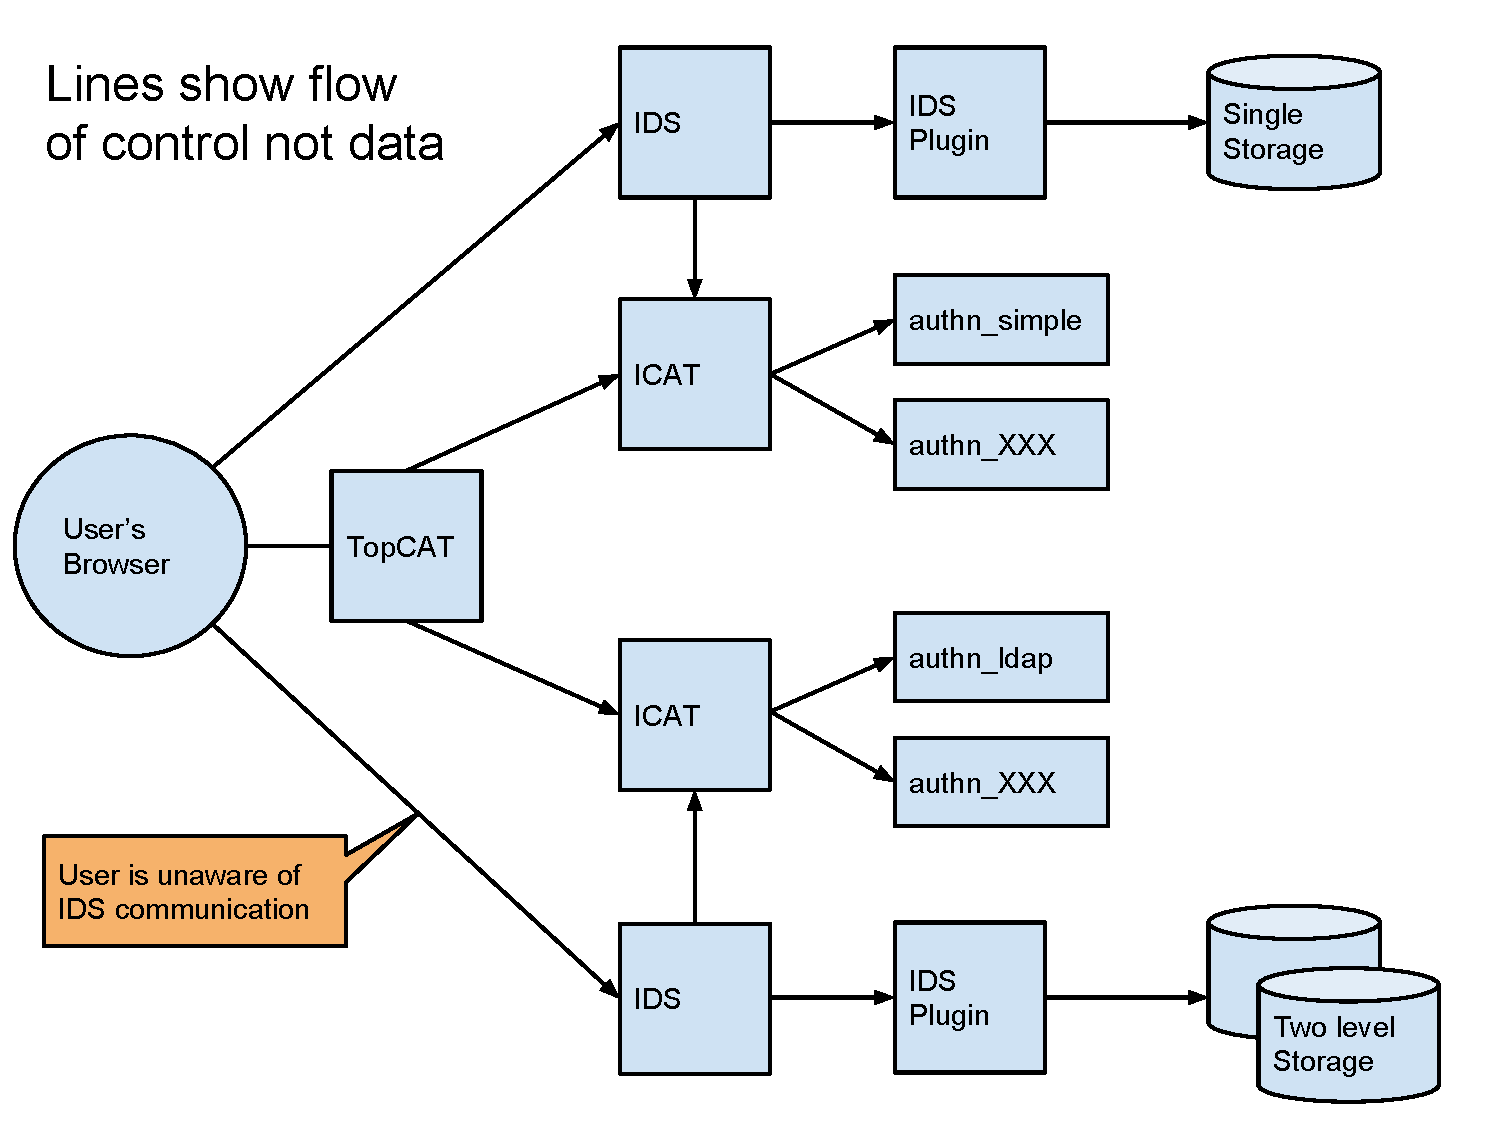
\includegraphics[scale=0.45]{ICATComponents.pdf}
    \caption{Block diagram showing some components}
    \label{fig:most_components}
\end{center}
\end{figure}
This is a web based GUI able to search across one or more ICAT server
instances and download data via the corresponding IDS server.
Figure~\ref{fig:most_components} shows how those ICAT components
mentioned so far might be used in conjunction with TopCAT.
The browser communicates with TopCAT which searches
in the ICAT server (here labelled simply as ICAT). It can provide
links to the IDS to download specific files located by their
metadata stored in the ICAT server. Each IDS sends messages to its
own ICAT server to make sure that any requested operations
are authorized. The IDS at the top of the figure is using an IDS
plugin which communicates with a single storage system. The IDS at
the bottom is using a plugin able to communicate with two level
storage: main and archive. Each ICAT server is shown with two
authenticators.

\section{Recent developments}
\subsection{TopCAT}
TopCat has already been mentioned as an established component however
it has recently had an overhaul so major that very few lines of old
code remain.  A major refactoring effort to replace the
GWT~\cite{ref:gwt} by AngularJS (version 1) and bootstrap began. This took
into account a requirements gathering exercise mostly based on
producing mockups and inviting comments. TopCAT now includes a
configurable set of data delivery mechanisms in addition to
http(s). One of these is the smartclient and the others are provided
by PollCAT both of which are described below.

\subsection{smartclient}
The smartclient is a small server packaged as a standalone
program. The user downloads this and starts the server which listens
for requests from TopCAT to download some data and queues a list of
Datafiles to be downloaded it then uses a number of threads to process
the queue so that it is doing a number of downloads from the IDS in
parallel to local storage. It is a convenient way to transfer a large
amount of data to your desktop machine.

\subsection{PollCAT}
When PollCAT is asked to perform a download it polls the IDS until
the data is ready, then transfers it to a location determined by a
plugin. Various plugins exist: for example to write to
PanFS~\cite{ref:panfs} or to a Globus Connect
Server~\cite{ref:globus_connect_server}. PollCAT is a third party
transfer mechanism.

\subsection{ICAT Job Portal}
The IJP~\cite{ref:ijp} was started in 2013. It makes use of the ICAT
server to locate data to process and can then submit and manage
compute jobs for interactive or batch processing. These jobs obtain
their data from the IDS and write new data into the IDS. A job may
record provenance information in the ICAT server for future
reference. Recently it was decided that this should also migrate
towards AngularJS and bootstrap. While prototyping this refactoring it
was realised that the code would have a lot in common with TopCAT;
TopCAT finds data and downloads it, the IJP finds data and submits it
for processing. It was then decided that the most efficient way
forward was to add a plugin mechanism to TopCAT, which has very
recently been done. The plugin mechanism added to TopCAT also allowed
a DOI (Digital Object Identifier) plugin to be written. This
communicates with another service to obtain DOIs.

\subsection{Dashboard}
The Dashboard is a web based GUI to give an overview of ICAT usage. It
subscribes to JMS messages transmitted by ICAT and IDS servers and
also itself makes calls to ICAT. The information is stored in a
database. The Dashboard has a number of displays to show information
about users and where they are and about volumes of downloaded
data. As a new component this was written from the beginning with a
Java back end and an AngularJS front end and will soon be released.

\section{Conclusion}
The CSMD data model has evolved and had proved to be applicable to
many different facilities. Because The ICAT family components have
been designed to be loosely coupled and to make use of plugins where
extensibility is required only around twenty person-years of
development effort has been invested into something which is meeting
the needs of many facilities. The use of lucene indexing by the ICAT
server has greatly improved the perfromance of TopCAT.

\section*{References}
\bibliographystyle{unsrt}
\bibliography{paper}

\end{document}
